% !TEX program = tectonic
\PassOptionsToPackage{table}{xcolor}
\documentclass[aspectratio=169,fontset=mac]{ctexbeamer}

\usepackage{fontspec}
\usepackage{ctex}
% \setCJKmonofont{STSong}
\usefonttheme{serif}            % 正文宋体，标题另设黑体

% 颜色（沿用报告）
\usepackage{xcolor}
\definecolor{ink}{HTML}{15384E}
\definecolor{ochre}{HTML}{A8702A}
\definecolor{rulecol}{HTML}{C9C2B2}
\definecolor{tinthdr}{HTML}{E9EEF0}
\definecolor{tintbox}{HTML}{F4F1E9}
\definecolor{textcol}{HTML}{17191C}

% Beamer 外观
\setbeamercolor{normal text}{fg=textcol}
\setbeamercolor{structure}{fg=ink}
\setbeamercolor{frametitle}{fg=ink}
\setbeamerfont{frametitle}{family=\sffamily,series=\bfseries,size=\large}
\setbeamercolor{itemize item}{fg=ink}
\setbeamercolor{itemize subitem}{fg=ink}
\setbeamertemplate{itemize item}{\small\raisebox{0.18ex}{\textcolor{ink}{\rule{0.7ex}{0.7ex}}}}
\setbeamertemplate{itemize subitem}{\textcolor{ink}{--}}
\setbeamertemplate{navigation symbols}{}
\setbeamertemplate{section in toc}{\textcolor{ink}{\inserttocsectionnumber.}~\inserttocsection}

% 标题下细规线
\setbeamertemplate{frametitle}{%
  \vskip0.6ex%
  \begin{beamercolorbox}[wd=\paperwidth,leftskip=0.045\paperwidth,rightskip=0.045\paperwidth]{frametitle}%
    \sffamily\bfseries\large\insertframetitle\par\vskip2pt%
    {\color{rulecol}\hrule height 0.9pt}%
  \end{beamercolorbox}%
}

% 页脚：当前段 · 页码
\setbeamercolor{footline}{fg=ink!75}
\setbeamertemplate{footline}{%
  \hbox to\paperwidth{\hskip0.045\paperwidth%
    \footnotesize\sffamily\color{ink!70}%
    \insertsection\hfill 面向边缘智能的 AIOS 设计与优化\hfill\insertframenumber\hskip0.045\paperwidth}%
  \vskip4pt%
}

% 表格
\usepackage{booktabs}
\usepackage{array}
\renewcommand{\arraystretch}{1.18}
\arrayrulecolor{rulecol}
\newcommand{\hdr}[1]{\textsf{\bfseries\color{ink}#1}}
\newcommand{\headrow}{\rowcolor{tinthdr}}

% 强调块
\setbeamercolor{block title}{fg=white,bg=ink}
\setbeamercolor{block body}{fg=textcol,bg=tintbox}
\usepackage{tikz}
\usepackage{pgfplots}
\pgfplotsset{compat=1.18}

\newcommand{\keyline}[1]{\par\vskip3pt\noindent\colorbox{tintbox}{\parbox{0.91\textwidth}{\color{ink}#1}}\par}

% 元信息
\title{面向边缘智能的 AIOS 设计与优化}
\subtitle{在 Starry 上承载 RK3588 网球拾取机器人视觉流水线}
\author{洪世金\quad 王乙凡\quad 徐子航}
\institute{队伍 Posad\quad 清华大学}
\date{2026 年 6 月}

\graphicspath{{./figures/}{../docs/figures/}}

\begin{document}

%
% 1 封面
\begin{frame}[plain]
\vfill
\begin{center}
{\sffamily\color{ink!75}\small 全国大学生计算机系统能力大赛\quad 操作系统设计赛\quad 功能挑战赛道}\\[10pt]
{\color{rulecol}\rule{0.86\textwidth}{1pt}}\\[16pt]
{\sffamily\bfseries\color{ink}\fontsize{24}{30}\selectfont 面向边缘智能的 AIOS 设计与优化}\\[10pt]
{\color{textcol}\large 在 Starry 上承载 RK3588 网球拾取机器人视觉流水线}\\[20pt]
{\color{ink!85}赛题 proj4（工程型，难度 A）\quad·\quad 目标平台 OrangePi 5 Plus / RK3588}\\[8pt]
{\color{ink!85}队伍 Posad\quad·\quad 清华大学\quad·\quad 洪世金、王乙凡、徐子航}\\[8pt]
{\color{ink!70}\small 2026 年 6 月}
\end{center}
\vfill
\end{frame}

%
% 2 目录
\begin{frame}{目录}
\vskip4pt
\begin{itemize}
\item \textbf{背景与目标}\quad 为什么在边缘做这件事，目标是什么
\item \textbf{系统使能}\quad 如何让机器人在 Starry 上运行
\item \textbf{性能优化}\quad 如何以 Linux 为基线追平性能
\item \textbf{增量与展望}\quad 本队增量、AI 方法与后续
\end{itemize}
\end{frame}

%
% 3 主要工作与结果
\begin{frame}{主要工作与结果}
\begin{itemize}
\item 相机经 NPU（片上神经网络推理加速器）检测、再驱动机械臂的完整拾球回路在 Starry 上跑通，检测结果与 Linux 一致。
\item 在与相机一致的 480×640 输入下，端到端推理由最初 30.6 ms 优化到 \textbf{11.75 ms}，与 Linux 的 11.4 ms 持平；另在 640×640 下由 162.7 降至 55.2 ms。
\item 实现块设备容错、USB 串口、reboot、RGA、JPU 等内核能力与硬件 PMU perf，其中五项已合并进上游，RGA 在审。
\end{itemize}
\keyline{两种输入尺寸计算量不同，各与对应尺寸的 Linux 基线比较；推理时延的结论是与 Linux 持平。}
\end{frame}

%
\section{背景与目标}

% 4 研究目标与实施阶段
\begin{frame}{研究目标与实施阶段}
将网球拾取机器人的内核由基于 C 的 Linux 迁移至以 Rust 实现的 Starry，工作分使能与优化两层，对应评审三阶段。
\vskip6pt
\begin{itemize}
\item 阶段一\quad 在板上启动 Starry 并跑通 NPU 推理。
\item 阶段二\quad 补齐 USB、串口等驱动与系统调用，让机械臂真正拾球。
\item 阶段三\quad 以 Linux 为基线开展性能优化。
\end{itemize}
\end{frame}

% 5 目标完成情况
\begin{frame}{目标完成情况}
\small
\begin{tabular}{@{}p{0.30\textwidth}p{0.10\textwidth}p{0.52\textwidth}@{}}
\toprule
\headrow \hdr{目标} & \hdr{状态} & \hdr{说明}\\
\midrule
阶段一　启动并跑通推理 & 完成 & 块设备容错使开发板稳定挂载，首次推理与 Linux 一致\\
阶段二　接齐外设并拾球 & 完成 & USB 串口接机械臂控制器，完整拾球回路跑通\\
阶段三　以 Linux 为基线优化 & 完成 & 480×640 下推理追平 Linux\\
启动、内存与能耗对照 & 进行中 & 精简内核具结构性优势，实测决赛前补\\
\bottomrule
\end{tabular}
\keyline{本工作有 640×640 与 480×640 两种输入尺寸，计算量不同，各与对应尺寸的 Linux 基线比较。}
\end{frame}

% 6 机器人及其工作回路
\begin{frame}{网球拾取机器人及其工作回路}
\centering
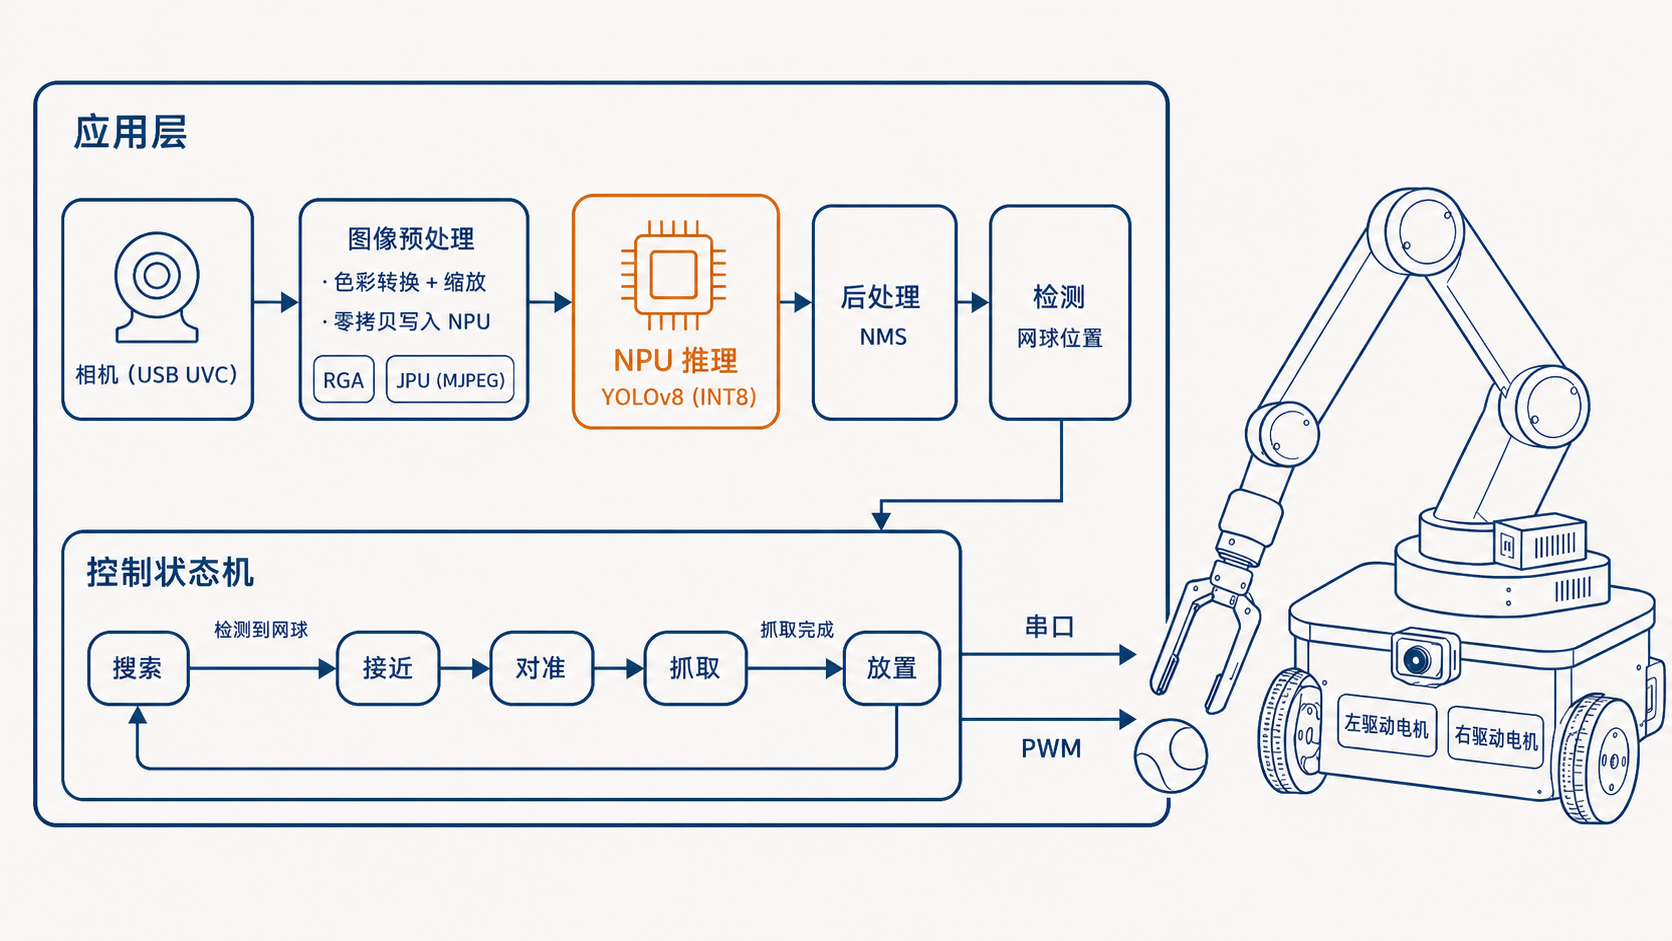
\includegraphics[width=0.82\textwidth,height=0.56\textheight,keepaspectratio]{app-workflow.png}
\par\vskip5pt
{\footnotesize 自主网球拾取机器人，移植自开源项目 pengzechen/aka-rk3588，原构建于基于 C 的 Linux。相机采集经图像预处理与 NPU 检测得到网球位置，控制状态机据此驱动机械臂与底盘。}
\end{frame}

% 7 迁移动机
\begin{frame}{迁移至 Starry 的动机}
\begin{columns}[T]
\begin{column}{0.48\textwidth}
\textbf{\color{ink}通用 Linux 在边缘的开销}
\begin{itemize}\small
\item 冗余的系统服务
\item 较长的执行路径
\item 较复杂的调度
\item 可观的内存占用
\end{itemize}
\end{column}
\begin{column}{0.48\textwidth}
\textbf{\color{ink}定制 Rust 内核的机会}
\begin{itemize}\small
\item 以 Rust 实现的精简内核
\item 面向场景深度定制
\item 更充分释放硬件
\end{itemize}
\end{column}
\end{columns}
\keyline{推理时延的目标是追平 Linux。启动、内存与能耗等维度尚未实测，列为后续工作，不预设结论；与类似项目的对照见后文对比页。}
\end{frame}

% 8 体系结构
\begin{frame}{软硬件体系结构}
\small
\begin{tabular}{@{}p{0.20\textwidth}p{0.74\textwidth}@{}}
\toprule
\headrow \hdr{层} & \hdr{内容}\\
\midrule
应用 & 网球拾取机器人程序，移植自 pengzechen/aka-rk3588\\
操作系统 & Starry，以 Rust 实现，构建于 ArceOS 组件\\
硬件 & RK3588（OrangePi 5 Plus）\\
\bottomrule
\end{tabular}
\vskip6pt
RK3588 的相关部件：大小核（A55×4 @1.8\,GHz 与 A76×4 @2.256\,GHz）；三核 NPU；RGA，二维图像缩放与色彩转换引擎，含多个功能各异的核；JPU，硬件 JPEG 解码单元。
\end{frame}

% 9 流水线阶段
\begin{frame}{视觉流水线的阶段划分}
\small
\begin{tabular}{@{}lp{0.74\textwidth}@{}}
\toprule
\headrow \hdr{阶段} & \hdr{职责}\\
\midrule
decode & 相机帧解码为 RGB。相机输出 YUYV 时直接转 RGB，输出 MJPEG（逐帧 JPEG）时需先解码，故分两路\\
letterbox & 等比缩放并填充到模型输入尺寸\\
inputs\_set & 写入 NPU，含缓存维护\\
run & NPU 一次前向推理\\
outputs\_get & 取回输出，并整理通道分块的张量排布\\
postprocess & 解码边框并做非极大值抑制\\
\bottomrule
\end{tabular}
\vskip4pt
\footnotesize 模型为 YOLOv8（单阶段实时目标检测网络）；RKNN 是瑞芯微 NPU 的模型格式与运行时，常见框架模型须经 rknn-toolkit2 转换才能加载。
\end{frame}

%
\section{系统使能}

% 10 启动
\begin{frame}{启动与根文件系统的接入}
\begin{columns}[T]
\begin{column}{0.48\textwidth}
\textbf{\color{ink}现象}\\[2pt]
\small 根文件系统所在 SD 卡由 dwmmc（板载 SD/eMMC 主机控制器）通道访问。注册块设备后启动停滞；中断路由与使能均无误，但该控制器未稳定拉起完成中断，中断驱动的完成等待因此持续等待。
\end{column}
\begin{column}{0.48\textwidth}
\textbf{\color{ink}做法}\\[2pt]
\small 完成等待超时即判定该设备中断不可用，转为轮询并对其后续传输沿用，中断正常的设备不受影响。
\end{column}
\end{columns}
\keyline{效果：启动由停滞转为稳定进入 shell。}
\end{frame}

% 11 reboot 与板端迭代
\begin{frame}{reboot 系统调用与板端迭代}
\begin{itemize}
\item \textbf{一键切换}\quad Linux 侧负责构建、上传资产与写入 FIT；reboot 后由 U-Boot 一次性引导 Starry，跑完后可回到 Linux。
\item \textbf{迭代效率}\quad Linux 与 Starry 的切换由手工操作或硬件插拔变为一条命令，缩短调试与复测路径。
\end{itemize}
\keyline{效果：Linux 与 Starry 的切换由人工上电、插拔或手工引导，收敛为一条命令触发的可复现流程。}
\end{frame}

% 12 动作外设驱动
\begin{frame}{动作外设驱动的接入}
\small
硬件上，机械臂经 USB 转串口接入舵机总线控制板，底盘两路直流电机经 DRV8833，由四路 PWM 控制方向与占空比。
\vskip4pt
\begin{columns}[T]
\begin{column}{0.48\textwidth}
\textbf{\color{ink}USB 串口}\\[2pt]
\begin{itemize}\footnotesize
\item rdrive 增加 USB 设备与接口 probe，按匹配结果绑定驱动。
\item CP210x 后端接入 Starry TTY 框架，复用行规程与文件接口。
\item 用户态保持 Linux 口径，仍通过 /dev/ttyUSB0 控制机械臂。
\end{itemize}
\end{column}
\begin{column}{0.48\textwidth}
\textbf{\color{ink}PWM 底盘}\\[2pt]
\begin{itemize}\footnotesize
\item 提供 Linux 兼容的 /sys/class/pwm 属性子集：export、period、duty\_cycle、enable。
\item RK3588 平台层按 FDT 应用 pinctrl，配置 pwmchip0/1/4/5 对应时钟与寄存器。
\item 底盘程序切换为 PWM 驱动后，不再占用唯一 UART3。
\end{itemize}
\end{column}
\end{columns}
\vskip4pt
\footnotesize 相机由 Starry 既有的 USB 主机栈在 USB3 端口枚举取流，进入流水线，非本队驱动。
\keyline{结果：机械臂经 /dev/ttyUSB0，底盘经 /sys/class/pwm，主流程中的动作控制都由 Starry 内核路径承载。}
\end{frame}

% 13 NPU 推理链路
\begin{frame}{NPU 推理链路的接入}
rknpu 设备节点与驱动是 Starry 既有部分。本队的工作：
\begin{itemize}
\item 修复 GEM（显存缓冲对象，图形子系统管理这类缓冲的机制）在映射时的缺页与销毁时的引用计数，任一都会让下次推理失败。
\item 以 rknn-toolkit2 将 YOLOv8 转为 RKNN 在板上加载。
\end{itemize}
\keyline{固定图输入下，首次推理的检测结果与 Linux 完全一致，机器人完整回路在 Starry 上闭合。}
\end{frame}

%
\section{性能优化}

% 14 剖析方法
\begin{frame}{剖析方法与测量工具}
\small
两侧采用同一份遵循 Linux ABI 的可执行文件、加载相同运行时与权重；干净运行与诊断运行分离；上游大同步后基线复测，主分位落在 ±2\%；每个数字独立复核。
\vskip5pt
基于硬件 PMU 的原生 perf（PR \#1395）对标 Linux 的 perf，读 CPU 的硬件计数器（周期、指令、缓存、分支），以每周期指令数与缓存计数判断负载受限于计算还是访存，并由按任务采集扩展到按核、再到感知大小核。
\vskip5pt
\footnotesize 观测能力：全链路分位与逐帧 CSV、冷启动四段拆分、拷贝与零拷贝 A/B、内核侧 ioctl 计时。
\end{frame}

% 15 Linux 基线 run
\begin{frame}{Linux 基线下 run 阶段是单帧时延主体}
\small
\begin{tabular}{@{}l*{4}{r}@{}}
\toprule
\headrow \hdr{阶段} & \hdr{平均} & \hdr{p50} & \hdr{p95} & \hdr{max}\\
\midrule
端到端 & 25.81 & 23.96 & 33.35 & 44.30\\
decode & 5.59 & 4.78 & 10.18 & --\\
letterbox（RGA）& 1.38 & 1.24 & 2.20 & 2.80\\
inputs\_set & 0.26 & -- & 0.45 & 7.50\\
\textbf{run（NPU）} & \textbf{15.42} & 14.82 & 19.35 & 28.18\\
outputs\_get & 1.30 & 1.43 & 1.54 & 2.24\\
postprocess & 1.06 & 1.19 & 1.25 & 1.86\\
\bottomrule
\end{tabular}
\keyline{run 约占除解码外各阶段之和的 79\%（15.42 / 19.4），卷积类算子占 NPU 时间约 72\%，故 run 由模型决定。消融排除了调度饥饿与内存带宽两项因素。}
\end{frame}

% 16 Starry 最初 6.3x
\begin{frame}{Starry 最初配置较 Linux 慢 6.3 倍，差距不在内核与 NPU}
\small
\begin{tabular}{@{}lrrr@{}}
\toprule
\headrow \hdr{阶段} & \hdr{Linux} & \hdr{Starry 最初} & \hdr{倍率}\\
\midrule
letterbox & 1.38 & 75.5 & 55×\\
run（NPU）& 15.42 & 71.1 & 4.6×\\
outputs\_get & 1.30 & 14.3 & 11×\\
端到端 & 25.81 & 162.7 & 6.3×\\
\bottomrule
\end{tabular}
\hfill（实时，模型输入 640×640，p50，单位 ms）
\vskip5pt
\small 内核计时显示提交 NPU 作业 0.360 ms、缓存维护 0.082 ms，相对 20 ms 量级推理微不足道。run 的实时 4.6× 是同一小核多项争用所致，固定图下 run 仅为 Linux 的 1.2 至 1.37 倍。
\end{frame}

% 17 根因
\begin{frame}{最初配置下线程串行于单个小核}
采集、解码、缩放与推理最初都落在 cpu0（一个 A55 小核）上相互串行。
\vskip6pt
成因：Starry 运行队列在派生与唤醒时不迁核，启动核是 cpu0，默认无负载均衡，而程序自身未设处理器亲和性，于是全部线程都落在 cpu0 上。
\vskip6pt
\footnotesize 另一层是缩放与色彩转换仍由 CPU 承担、尚未用上 RGA，留到第三个杠杆。
\end{frame}

% 18 大核放置
\begin{frame}{将推理绑定至大核}
\small
\begin{tabular}{@{}lrrr@{}}
\toprule
\headrow \hdr{阶段} & \hdr{最初} & \hdr{绑定 A55} & \hdr{绑定 A76}\\
\midrule
run（NPU）& 71.1 & 71.2 & 24.5\\
letterbox & 75.5 & 74.9 & 26.4\\
outputs\_get & 14.3 & 14.3 & 2.7\\
端到端 & 162.7 & 162.8 & 55.2\\
\bottomrule
\end{tabular}
\hfill（实时，模型输入 640×640，p50，单位 ms）
\vskip5pt
\small 核驻留直方图显示推理由 cpu0 迁到 cpu4，亲和性被遵从；采集帧率 10.9 升至 17.7。此时相对 Linux 25.8 仍约 2.1 倍，残余主要在 letterbox（仍走 CPU）。亲和性须在 NPU 与 USB 初始化之后设置，否则二级核挂起。
\end{frame}

% 19 整数路径
\begin{frame}{以整数路径取回输出}
\small
NPU 输出为 INT8，原本每帧约四十万个数全部反量化。改为整数域阈值先筛掉背景单元，只对存活的数十个反量化；因反量化单调、整数域比较等价，结果不变，285 张图与浮点路径逐一一致。outputs\_get 由约 12 ms 降到约 1 ms。
\vskip5pt
\textbf{模型层准备}（与整数路径正交）：模型导出为 480×640，省方形填充、letterbox 计算量随之下降；SiLU 换 ReLU，NPU 原生算子，run 快约 2.5 倍。
\keyline{480×640 下，整数输出、大核放置与 ReLU 三者叠加，端到端 11.75 ms，与 Linux 11.4 持平。}
\end{frame}

% 20 RGA 零拷贝
\begin{frame}{以 RGA 零拷贝合并解码与缩放}
\small
重活迁往大核后，相机帧的 YUYV→RGB 色彩转换（decode）成为 CPU 上最高的一项。RGA 同时承担 decode 与缩放填充，并在关闭 IOMMU（设备侧地址翻译部件）后以物理地址直通写入 NPU 输入缓冲，各阶段间不再拷贝。
\vskip5pt
结果：decode p50 0.776 ms、inputs\_set 归零；在 11.75 的基础上端到端进一步降至 9.65 ms，约 28 fps 的吞吐受相机供帧速率限制。
\keyline{9.65 相对 11.75 的下降来自 RGA 接管前处理；持平结论以同尺寸的 11.75 与 11.4 为准。}
\end{frame}

% 20b 以 JPU 硬件解码 MJPEG
\begin{frame}{以 JPU 硬件解码相机的 MJPEG}
\small
相机原生以 MJPEG（逐帧 JPEG 压缩）输出，须先解码为像素。前述各步在 YUYV 模式下由 RGA 直接转色彩；改用相机原生的 MJPEG 模式后，这一解码若由 CPU 承担单帧约 25 ms，会重新主导时延。
\vskip5pt
接入 JPU 后，MJPEG 由硬件解码为 NV12（单帧约 1 ms），再交 RGA 转色彩、直写 NPU 输入缓冲，整条 MJPEG$\to$JPU$\to$RGA$\to$NPU 全程零拷贝。
\keyline{在机器人实际使用的 MJPEG 模式下，端到端 p50 为 9.06 ms，约 29 fps（受相机供帧速率限制），与 YUYV 路径约 9 ms 相当。}
\end{frame}

% 21 优化历程（原生历程图）
\begin{frame}{各步优化的端到端时延}
\centering
\begin{tikzpicture}
\begin{semilogyaxis}[
  width=0.92\textwidth, height=0.58\textheight,
  ymin=7, ymax=240, log basis y=10,
  ytick={10,20,50,100,200}, yticklabels={10,20,50,100,200},
  ylabel={端到端 p50（ms）}, ylabel style={font=\scriptsize},
  yticklabel style={font=\scriptsize},
  xmin=0.6, xmax=6.4, xtick={1,2,3,4,5,6},
  xticklabels={{YOLOv8 640×640},{绑大核},{降 480×640},{免反量化},{RGA 零拷贝},{JPU 解码}},
  xticklabel style={font=\scriptsize\sffamily},
  axis line style={rulecol}, tick style={rulecol},
  nodes near coords, point meta=explicit symbolic,
  every node near coord/.append style={font=\scriptsize\bfseries, color=ink, anchor=south, yshift=2pt},
  clip=false,
]
\addplot[ochre, dashed, thick, forget plot] coordinates {(0.8,25.8) (2.5,25.8)};
\addplot[ochre, dashed, thick, forget plot] coordinates {(2.6,11.4) (6,11.4)};
\addplot[ink, very thick, mark=*, mark options={fill=white,draw=ink,line width=0.8pt}]
  coordinates {(1,162.7)[162.7] (2,55.2)[55.2] (3,30.6)[30.6] (4,11.75)[11.75] (5,9.65)[9.65] (6,9.06)[9.06]};
\end{semilogyaxis}
\end{tikzpicture}
\par\vskip1pt
{\footnotesize 实线为 Starry 各步优化，赭色虚线为对应尺寸的 Linux 基线（640×640 为 25.8 ms，480×640 为 11.4 ms）。11.75 与 Linux 11.4 持平；9.65 为再加 RGA 零拷贝的 Starry 侧结果，完整流水线与 Linux 的对照见后文。}
\end{frame}

% 22 负面结果
\begin{frame}{无收益的尝试及其边界}
\begin{itemize}
\item \textbf{NPU 张量零拷贝}\quad 把输出重排从内核搬到用户态，单核上只换位置不减开销，总时延反升约 22\%（诊断口径）；多核并发取输出时才划算。
\item \textbf{第三个 NPU 核}\quad 算子集中在一核，另两核近空闲；可留作三重缓冲或并行跑另一模型。
\item \textbf{锁定调频}\quad NPU 全程已稳定 1.0\,GHz，故无变化。
\end{itemize}
\end{frame}

%
\section{增量与展望}

% 23 RGA 驱动
\begin{frame}{RGA 驱动的实现}
\small
\textbf{两层实现}：底层 RGA2 寄存器级驱动，含开时钟、解软复位、主模式，以及提交、轮询、应答、复位的状态机；上层把 librga 的请求结构 rga\_req 按真实二进制布局在内核镜像并翻译，故无需改动机器人程序。
\vskip4pt
\textbf{三处障碍}：相机与 NPU 缓冲分属不同分配器、句柄无法直接导入，改按物理地址导入；设备树三个 RGA 核中有一个不支持所需操作，初版误锁致提交失败，改为按操作选核；librga 每个请求都填一个表示不旋转的单位矩阵，驱动初版误判为非法旋转参数而拒绝，改为仅当旋转模式非零才解析。
\keyline{五项操作逐像素 CRC 自测通过，PR \#1388。}
\end{frame}

% 24 JPU 驱动
\begin{frame}{JPU 驱动的实现}
JPU 以 /dev/mpp\_service 暴露，遵循瑞芯微多媒体框架 MPP 的用户态接口，为相机的 MJPEG 模式提供硬件解码。标准解码测试 mpi\_dec\_test 的输出与 Linux 逐字节一致，校验和同为 2712426383。
\vskip5pt
接入机器人程序后，JPU 与 RGA、NPU 共用同一段 dma-heap 缓冲，构成前述的 MJPEG$\to$JPU$\to$RGA$\to$NPU 零拷贝流水线（端到端 9.06 ms）。
\vskip5pt
\footnotesize RGA 与 JPU 都采用既有库的真实接口（librga、MPP）而非自定义 ioctl，这是不改机器人程序即可对接的前提。
\end{frame}

% 24b 完整零拷贝流水线与 Linux 的对照
\begin{frame}{完整零拷贝流水线与 Linux 的对照}
\small
同一开发板、同一程序，MJPEG$\to$JPU$\to$RGA$\to$NPU 全硬件零拷贝在两侧均已跑通。逐阶段 p50（480×640）：
\vskip3pt
\begin{center}\footnotesize
\begin{tabular}{lcc}
\toprule
阶段（p50，ms）& Linux & Starry\\
\midrule
解码（JPU 与 RGA）& 2.11 & 1.21\\
run（NPU）& 10.89 & 4.76\\
端到端（帧到检测）& 13.89 & 9.06\\
\bottomrule
\end{tabular}
\end{center}
\vskip3pt
中位差异来自调频而非两侧硬件的快慢：Starry 不降频，Linux 默认 ondemand 在持续负载下把 NPU 降频（固定图连测 Linux 4.7$\to$10.6、Starry 稳定 4.8）。同一时钟下 NPU 本就相当，与 480×640 下 11.75 与 11.4 的持平印证，切到 performance 即追平。
\keyline{代价在尾部：Starry 端到端最坏 487 ms（Linux 22），丢帧约一成，冷启动更慢；常驻内存反更省（19 比 31 MB），检测精度一致。}
\end{frame}

% 25 基础版本与增量
\begin{frame}{基础版本与增量贡献}
\footnotesize
基础版本：内核 rcore-os/tgoskits @ dev（fork 自 Starry-OS/StarryOS，基线 commit 73409e079）；应用 pengzechen/aka-rk3588；模型工具 rknn-toolkit2。
\vskip4pt
\begin{tabular}{@{}p{0.46\textwidth}p{0.46\textwidth}@{}}
\toprule
\headrow \hdr{贡献} & \hdr{上游提交}\\
\midrule
硬件 PMU perf & PR \#1395，已合并\\
USB 串口驱动 & PR \#1378，已合并\\
reboot 系统调用 & PR \#1358，已合并\\
rknpu 整合与 GEM 修复 & PR \#1351、\#1364，已合并\\
RGA 驱动 & PR \#1388，开放中\\
JPU、块设备容错、PWM、profile-rknpu、负载均衡器原型 & 待提交\\
\bottomrule
\end{tabular}
\end{frame}

% 26 与类似项目对比
\begin{frame}{与类似项目的对比}
\small
\textbf{\color{ink}唯一同口径可比}\quad 与同机 Linux：同机、同模型、同 NPU、同 480×640 输入，端到端 11.75 ms 与 11.4 ms 持平。其余项目硬件、模型与口径各异，推理时延不具可比性，仅作定性定位。
\vskip5pt
\scriptsize
\begin{tabular}{@{}p{0.19\textwidth}p{0.16\textwidth}p{0.12\textwidth}p{0.19\textwidth}p{0.16\textwidth}@{}}
\toprule
\headrow \hdr{项目} & \hdr{系统/语言} & \hdr{硬件量级} & \hdr{加速器接入} & \hdr{真机闭环}\\
\midrule
本工作 & Starry / Rust & RK3588 SoC & 自实现 rknpu 加 RGA/JPU & 完整机器人回路\\
Ariel-ML & Ariel OS / Rust & 微控制器 & 多核 CPU，无加速器 & 推理，非机器人\\
mtx512/rk3588-npu & Linux / C & RK3588 SoC & 直驱 NPU（逆向）& 矩阵乘验证\\
OSComp proj311 & ArceOS / Rust & 飞腾派 & 未接 NPU & HID 到电机\\
工业 RKNPU2 & Linux / C++ & RK3588 SoC & 官方闭源运行时 & 官方部署路径\\
\bottomrule
\end{tabular}
\vskip3pt
\footnotesize 按是否接专用 NPU、硬件量级与是否真机机器人闭环定位，不比较延迟。工业 RKNPU2 是本工作所复现的生产路径（自写设备层并对齐 librga 与 MPP 真实接口）。详见随附对比分析文档。
\end{frame}

% 27 队员分工
\begin{frame}{队员分工}
\small
\begin{tabular}{@{}lp{0.78\textwidth}@{}}
\toprule
\headrow \hdr{成员} & \hdr{负责模块与交付物}\\
\midrule
洪世金 & 剖析方法与基线、用户态优化、RGA 与 JPU 驱动、硬件 PMU perf、块设备完成路径容错、报告撰写\\
王乙凡 & USB 串口驱动、reboot 系统调用、PWM 驱动\\
徐子航 & 模型训练与数据集准备、系统测试与现场验证\\
\bottomrule
\end{tabular}
\end{frame}

% 28 进度
\begin{frame}{开发进度与完成情况}
\small
\begin{tabular}{@{}lp{0.66\textwidth}l@{}}
\toprule
\headrow \hdr{阶段} & \hdr{主要工作} & \hdr{状态}\\
\midrule
剖析口径搭建 & 在同一份程序与内核中补齐观测能力 & 完成\\
Linux 基线 & 在板上完成基线深度剖析 & 完成\\
Starry 使能 & 块设备容错，首次跑通 NPU 推理 & 完成\\
本体接入 & USB 串口、reboot、相机取流 & 完成\\
用户态优化 & 大核放置、整数输出、RGA 零拷贝 & 完成\\
内核能力 & 加速器驱动、硬件 perf、负载均衡器原型 & 完成\\
\bottomrule
\end{tabular}
\end{frame}

% 29 AI 使用说明
\begin{frame}{AI 使用说明}
\small
\begin{tabular}{@{}p{0.40\textwidth}p{0.32\textwidth}p{0.20\textwidth}@{}}
\toprule
\headrow \hdr{工具} & \hdr{大模型} & \hdr{用途}\\
\midrule
Claude Code & Claude Opus 4.8 与 Claude Sonnet 4.6 & 生成、调试、分析、编排、文档\\
ChatGPT 图像生成 & GPT-4o 图像生成 & 仅方法论示意图\\
\bottomrule
\end{tabular}
\vskip5pt
\footnotesize 使用场景：检索、生成、调试、日志整理、撰写。AI 在规格内实现，架构、正确性判据与采纳由队员决定，每个数字对照原始日志独立复核，交互记录摘要随附材料给出。
\end{frame}

% 30 方法论
\begin{frame}{AI 辅助开发方法与正确性保障}
\begin{columns}[c]
\begin{column}{0.46\textwidth}
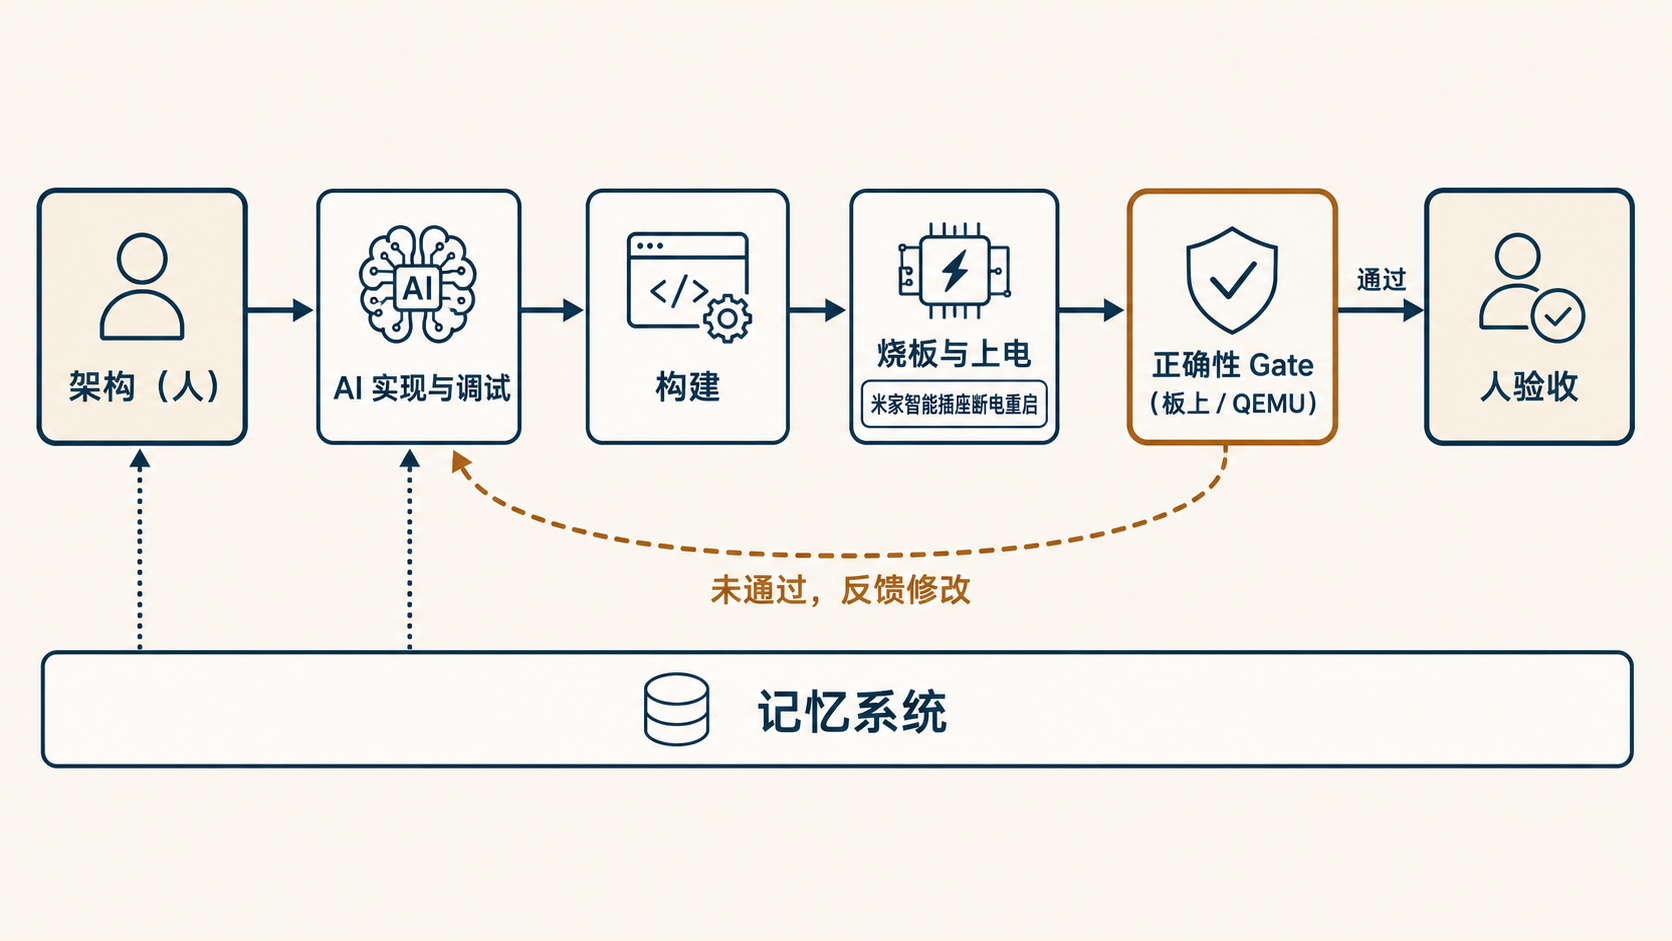
\includegraphics[width=\textwidth]{methodology-loop.png}
\end{column}
\begin{column}{0.50\textwidth}
\footnotesize
\begin{itemize}
\item \textbf{机器可判定的闸门}：RGA 逐像素 CRC、JPU 校验和、285 张图整数与浮点一致、QEMU 与板上用例。
\item \textbf{真机闭环}：内核挂起堵死自动迭代，米家智能插座据此远程断电重启，reboot 切换 Linux 与 Starry。
\item \textbf{测量驱动与对抗式验证}：结论须经独立复核反驳，“同一份 ELF 上推理快过 Linux”的设想已被测量否定。
\item \textbf{记忆与规格先行}；人掌控架构与验收，可在无 AI 下解释关键设计并现场修改。
\end{itemize}
\end{column}
\end{columns}
\end{frame}

% 31 主要贡献与创新点
\begin{frame}{主要贡献与创新点}
\begin{itemize}
\item 完整机器人回路在一个研究型 Rust 操作系统上跑通。
\item 端到端推理在 480×640 下追平 Linux（11.75 与 11.4 ms），另在 640×640 下由 162.7 降至 55.2。
\item RGA、JPU、硬件 perf 等已实现，多项合并上游。
\item 提出并实践了一套机器可判定闸门加真机闭环的 AI 辅助操作系统开发方法。
\end{itemize}
\end{frame}

% 32 后续与可复现
\begin{frame}{后续工作与可复现性}
\textbf{\color{ink}后续}
\begin{itemize}\small
\item 系统：架构感知调度免去手动绑核；NPU 三核并发，突破设备锁串行。
\item 应用：ACT 动作分块模仿学习、语音输入、接近百分之百的抓取策略、里程计记住回收桶位置。
\end{itemize}
\vskip2pt
\textbf{\color{ink}可复现}\quad{\small 直连网络与串口、U-Boot 引导、无板时容器内 QEMU、纯标准库渲染剖析图。}
\vskip4pt
\footnotesize 材料：设计方案 PDF、演示视频、本片与仓库链接。
\end{frame}

\end{document}
